% Unofficial Georgia Tech Math Poster Template
% based on the unnoficial Georgia Tech Psychology Poster Template, in turn based on
% based on
% https://github.com/k4rtik/uchicago-poster
% a fork of https://github.com/anishathalye/gemini

\documentclass[final]{beamer}

% ====================
% Packages
% ====================

\usepackage[T1]{fontenc}
\usepackage{lmodern}
\usepackage[size=custom,width=96,height=72,scale=1.0]{beamerposter}%\usetheme{gemini}

% ===== Override Gemini Green With Blue =====

\definecolor{PosterBlue}{RGB}{0, 51, 153}     % main blue
\definecolor{LightBlue}{RGB}{230, 240, 255}   % subtle background blue

% Background
\setbeamercolor{background canvas}{bg=white}

% Title bar (top banner)
\setbeamercolor{headline}{bg=PosterBlue, fg=white}
\setbeamercolor{title}{fg=white, bg=PosterBlue}
\setbeamercolor{frametitle}{fg=white, bg=PosterBlue}

% Regular blocks
\setbeamercolor{block title}{fg=white, bg=PosterBlue}
\setbeamercolor{block body}{bg=LightBlue, fg=black}

% Alert blocks
\setbeamercolor{alertblock title}{fg=white, bg=PosterBlue}
\setbeamercolor{alertblock body}{bg=LightBlue, fg=black}

% Footer bar
\setbeamercolor{footline}{fg=white, bg=PosterBlue}

% \usecolortheme{gemini}
\usepackage{amsmath, amssymb, amsthm}
\usepackage{graphicx}
\usepackage{xcolor}
\usepackage{booktabs}
\usepackage{doi}
\usepackage{natbib}
\usepackage[patch=none]{microtype}
\usepackage{tikz}
\usepackage{mathtools}
\usepackage{pgfplots}
\pgfplotsset{compat=1.18}
\usepackage{anyfontsize}
\usepackage{multirow} % Allows diagrams to take up multiple rows
\usepackage{wrapfig}

% \renewcommand{\arraystretch}{1.4} % Stretches tables vertically for more white space
\usepackage{mathrsfs} % for script N lol
\setlength{\tabcolsep}{15pt} % Adjusts space between text and column edges

\usepackage{url}
\urlstyle{same}

\newcommand{\R}{\mathbb{R}}
\newcommand{\N}{\mathbb{N}}
\newcommand{\Z}{\mathbb{Z}}
\newcommand{\C}{\mathbb{C}}
\newcommand{\Q}{\mathbb{Q}}
\newcommand{\F}{\mathbb{F}}
\newcommand{\Aut}{\mathrm{Aut}}

\pdfstringdefDisableCommands{%
	\def\translate#1{#1}%
	
}

% ====================
% Lengths
% ====================

% If you have N columns, choose \sepwidth and \colwidth such that
% (N+1)*\sepwidth + N*\colwidth = \paperwidth
\newlength{\sepwidth}
\newlength{\colwidth}
\setlength{\sepwidth}{0.025\paperwidth}
\setlength{\colwidth}{0.3\paperwidth}

%\setbeamerfont*{itemize/enumerate body}{size=\normal}
\setbeamerfont*{itemize/enumerate subbody}{parent=itemize/enumerate body}
\setbeamerfont*{itemize/enumerate subsubbody}{parent=itemize/enumerate body}

\setbeamercolor{block title example}{fg=blue}
\setbeamercolor{itemize item}{fg=blue}
\setbeamertemplate{caption}[numbered]


\newcommand{\separatorcolumn}{\begin{column}{\sepwidth}\end{column}}

% ====================
% Title
% ====================

\title{Convolutional Neural Network \\ for Cardiac Arrhythmia Detection from ECG Signals}

\author{Alexander Nwanganga\texorpdfstring{$^\text{1}$}{} \and Prof. Ackley Will (PhD)\texorpdfstring{$^\text{1}$}{}}

\institute[shortinst]{$^\text{1}$Andrews University}

% ====================
% Footer (optional)
% ====================


% (can be left out to remove footer)

% ====================
% Logo (optional)
% change logos in header by replacing the png files
% ====================


% ====================
% Body
% ====================

% --- Show a real title/header bar ---
\setbeamertemplate{headline}{
	\begin{beamercolorbox}[wd=\paperwidth,ht=8cm,dp=1.2cm]{headline}
		\vfill
		\centering
		{\fontsize{60}{70}\bfseries\inserttitle\par}
		\vspace{0.3cm}
		{\large\insertauthor\par}
		{\large\insertinstitute\par}
		\vfill
	\end{beamercolorbox}
}


\begin{document}
	\addtobeamertemplate{headline}{}
	{
		\begin{tikzpicture}[remember picture, overlay]
			\node [anchor=north west, inner sep=3cm] at ([xshift=3.5cm,yshift=2cm]current page.north west)
			{
\includegraphics[height=7cm]{imagens/au_seal.png}};
			\node [anchor=north east, inner sep=3cm] at ([xshift=0.5cm,yshift=1cm]current page.north east)
			{
\includegraphics[height=5cm]{imagens/Untitled.png}};
		\end{tikzpicture}
	}
	
	\begin{frame}[t]
		\begin{columns}[t]
			\separatorcolumn
			
			\begin{column}{\colwidth}
				\begin{block}{Overview} 
					
					Cardiac arrhythmia accounts for the largest percentage of premature deaths in the United States. These are heart conditions characterized by uncoordinated electrical pulses in the heart. These pulses can be read through ECG readings and diagnosed by a medical professional. Due to the intermittent and irregular nature of its symptoms, reliable detection is difficult, especially in short or noisy signals. In this work, we investigate machine learning approaches for the automated classification of various types of cardiac arrhythmias. With an emphasis on classifying the type of arrhythmia given a limited signal duration.
					  
				
				
					
				\end{block}
				
				\bigskip
				
				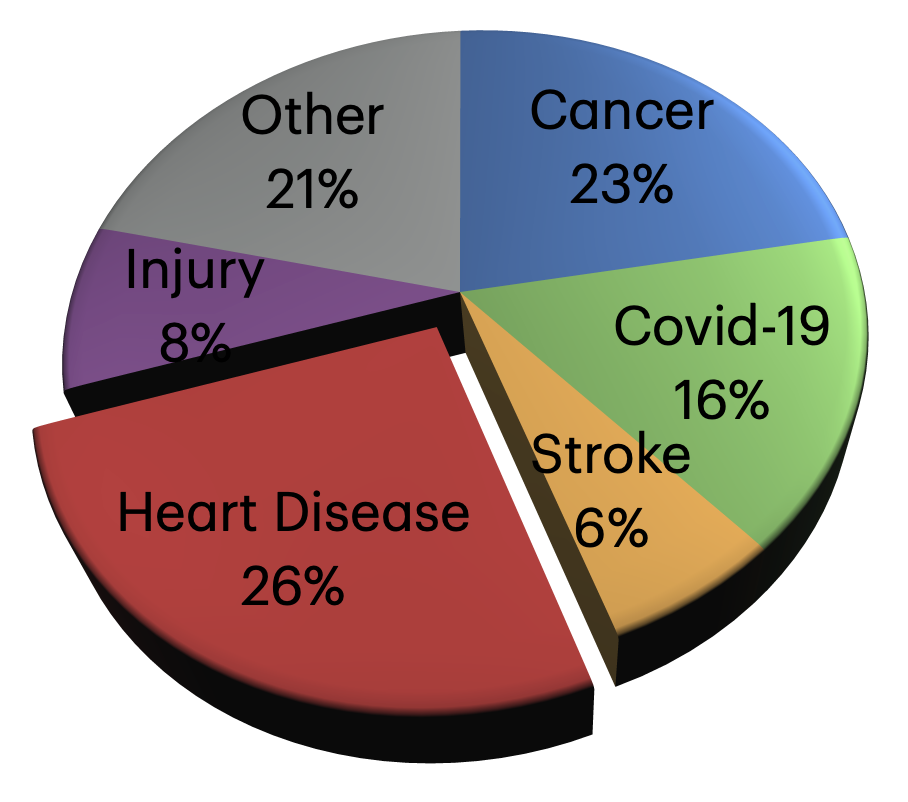
\includegraphics[width=0.4\textwidth]{imagens/Pie_Chart.png}
				\includegraphics[width=0.55\textwidth]{imagens/ECG_signal.png} 
				{\small \textbf{Fig. 1} Leading causes of death in the U.S.  \textbf{Fig. 3} Sample ECG signal from MIT-BIH database}
				
				
				\begin{block}{About the Dataset}
					The dataset used in this study was sourced from the PhysioNet site and contains an open-source download of a dataset with the following characteristics: 
					
					\bigskip
					
					\begin{itemize}
						\item MIT-BIH Arrhythmia Database
						\item 12-lead ECGs 
						\item Selected 9 of 63 classes for comparison against baseline paper
						\item Consists of 45,152 patient ECGs
						\item ECG segments are 10 sec length 
						\item 500 Hz sampling rate
						\item Each class has anywhere from 500 to 9000 samples
					\end{itemize}
					
				\end{block}
				
				\smallskip
				
				\begin{exampleblock}{Preprocessing}
					Developed a flexible Python preprocessing pipeline to standardize labels and restructure the dataset automatically traversing the dataset tree, operating on paired .hea and .mat files with shared basenames.Used the WFDB library (wfdb.rdheader) to:
					
					\begin{itemize}
						\item Extract classification metadata
						\item Identify sampling frequency and lead information
						\item Removed incomplete or improperly labeled records.
					\end{itemize}
					
					
					\bigskip
					
					Label Standardization
					
					\smallskip
					
					\begin{itemize}
						\item Extracted numeric diagnostic codes from header comment lines.
						\item Cross-referenced codes with the 'SNOMED CT' clinical terminology table.
						\item Converted numerical identifiers into clinically meaningful arrhythmia labels.
						\item Reorganized records into class-specific directories (hierarchical dataset structure).
					\end{itemize}
				
				\bigskip
				
					Test/Training Split: 
					
					\begin{itemize}
						\item Applied stratified 80/20 split to preserve class distributions and randomized dataset prior to partitioning.
					\end{itemize}
					
					\vspace{0.5em}
					
				
					
				\end{exampleblock}
				
			\end{column}
			
			\separatorcolumn
			
			\begin{column}{\colwidth}
				
				\begin{block}{Classical Model: 1-D Convolutional Neural Network}
					
					
					
					\begin{itemize}
						\item 1D Convolutional Neural Networks (CNNs) effectively learn and extract discriminative features directly from raw ECG waveforms. 
						\item Well-suited for time-series data, enabling detection of temporal patterns such as normal sinus rhythm vs. arrhythmic activity.
						\item Convolutional layers apply learnable filters to capture local waveform features (e.g., QRS complex morphology, rhythm irregularities).
						\item Pooling layers reduce feature dimensionality, improve computational efficiency, and enhance robustness to small temporal variations.
					\end{itemize}
					
					\bigskip
					
					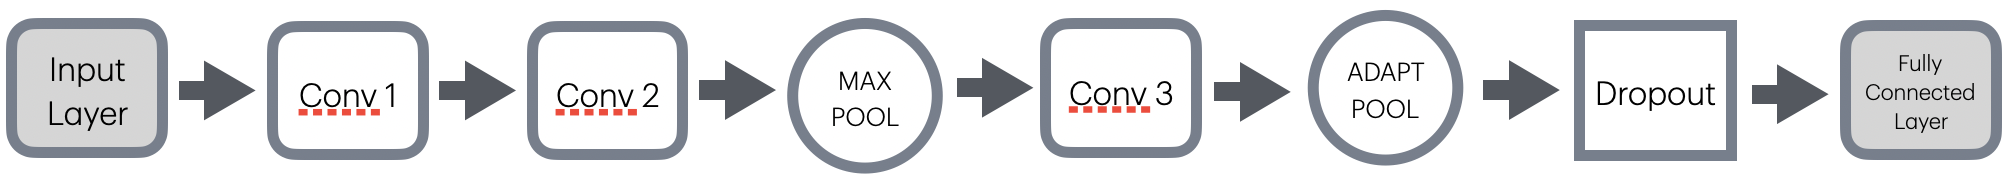
\includegraphics[width=1\textwidth]{imagens/Test_Model.png}
					
					\bigskip
					
					%\caption{Experimental Model: 1-D CNN Architecture}					
					
					\bigskip
					
					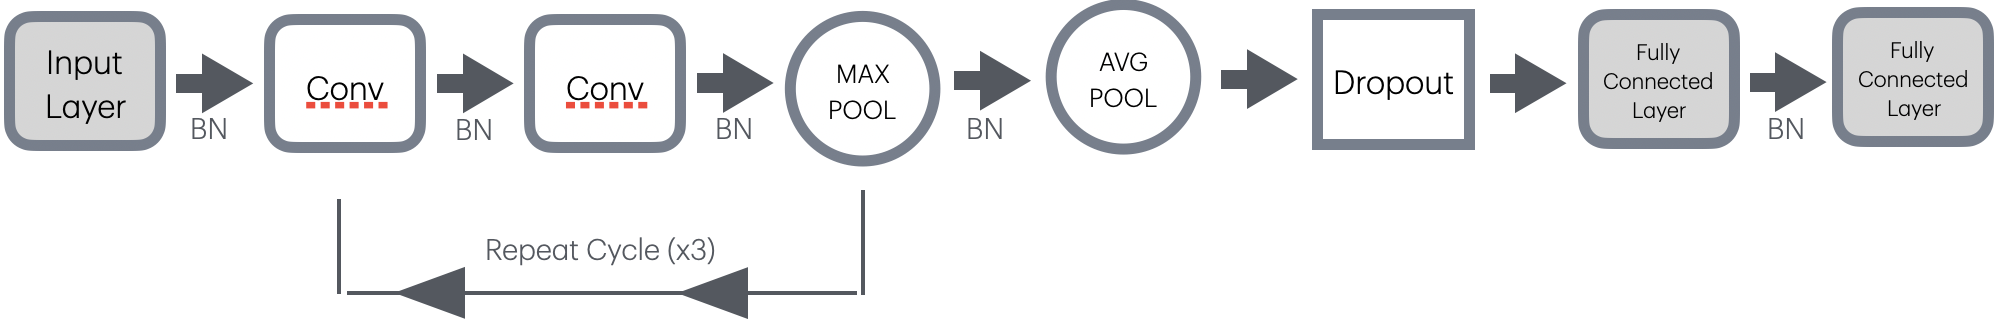
\includegraphics[width=1\textwidth]{imagens/Base_Model.png}
					{\small \textbf{Fig. 2} Baseline Model -1D CNN Architecture}
						
					\bigskip
					
					The architecture is modular and includes tunable hyperparameters:
					\begin{itemize}
						\item Number of filters: F
						
						\item Kernel size: k
						
						\item Dropout rate: p
						
						\item Batch size
						
					\end{itemize}	
						
					\bigskip
						
					This flexibility enables systematic performance optimization.	
					
					\bigskip
					
					For an input ECG signal $x[n]$, a 1D convolutional layer computes:
					
					\[
					y_j[n] = \sum_{i=1}^{C} \sum_{m=0}^{k-1} w_{j,i}[m] \, x_i[n-m] + b_j
					\]	
						
						
					\smallskip
						
					
					\begin{itemize}
						\item $k$ = kernel size
						\item $w_{j,i}$ = learned filter weights
						\item $b_j$ = bias
						\item $y_j[n]$ = output feature map
					\end{itemize}
					
					\smallskip
					
				
				\end{block}
				
				\begin{exampleblock}{Results}
					Training both models on several different seeds resulted in the following performance scores:
					\begin{table}[h]

						\bigskip
						
						\centering
						\caption{Test Model Performance Across Random Seeds}
						\label{tab:test_model}
						\begin{tabular}{lcccccc}
							\hline
							Seed & 13 & 23 & 33 & 43 & 53 & Avg \\ 
							\hline
							Accuracy  & 99.77\% & 99.87\% & 99.86\% & 99.87\% & 99.84\% & $99.84\%\pm0.04\%$ \\
							Precision & 99.06\% & 99.93\% & 99.85\% & 99.88\% & 99.79\% & $99.70\%\pm0.36\%$ \\
							Recall    & 99.62\% & 99.83\% & 99.80\% & 99.85\% & 99.80\% & $99.78\%\pm0.09\%$ \\
							F1 Score  & 99.33\% & 99.80\% & 99.82\% & 99.86\% & 99.79\% & $99.72\%\pm0.22\%$ \\
							\hline
						\end{tabular}
						
					\end{table}
					
					\begin{table}[h]
						\centering
						\caption{Base Model Performance Across Random Seeds}
						\label{tab:base_model}
						\begin{tabular}{lcccccc}
							\hline
							Seed & 13 & 23 & 33 & 43 & 53 & Avg \\ 
							\hline
							Accuracy  & 96.31\% & 99.92\% & 81.67\% & 83.13\% & 89.23\% & $90.05\%\pm7.99\%$ \\
							Precision & 70.08\% & 99.79\% & 28.40\% & 58.99\% & 56.82\% & $62.82\%\pm25.76\%$ \\
							Recall    & 72.64\% & 99.74\% & 33.12\% & 66.66\% & 64.08\% & $67.25\%\pm23.77\%$ \\
							F1 Score  & 70.96\% & 99.77\% & 29.66\% & 52.87\% & 57.58\% & $62.17\%\pm25.77\%$ \\
							\hline
						\end{tabular}
						
					\end{table}
				
				\end{exampleblock}
				
			\end{column}
			
			\separatorcolumn
			
			\begin{column}{\colwidth}
				
				\begin{block}{Quantum Convolutional Neural Network}
					\begin{itemize}
						\item \textbf{Classical Preprocessing} - In this step our goal is to reduce dimensional while preserving diagnostic structure. By decreasing the over 1000 samples from 2 sec long recordings into a feature map with only C number of components.
						\item \textbf{Quantum Feature Encoding} - Each classical feature is encoded into a qubit via parameterized rotations.
						\item \textbf{Quantum Convolutional Layers} - Apply two quibit gates and leverages entanglement to extract hierarchical quantum features and capture correlations between neighboring qubits. These are comparable to spatial features in classical CNNs.
						\item \textbf{Quantum Pooling Layers} - Applies controlled rotations effectively compressing quantum information further. 
					\end{itemize}
					%%%%%%%%%%%%%%%        
					\centering
					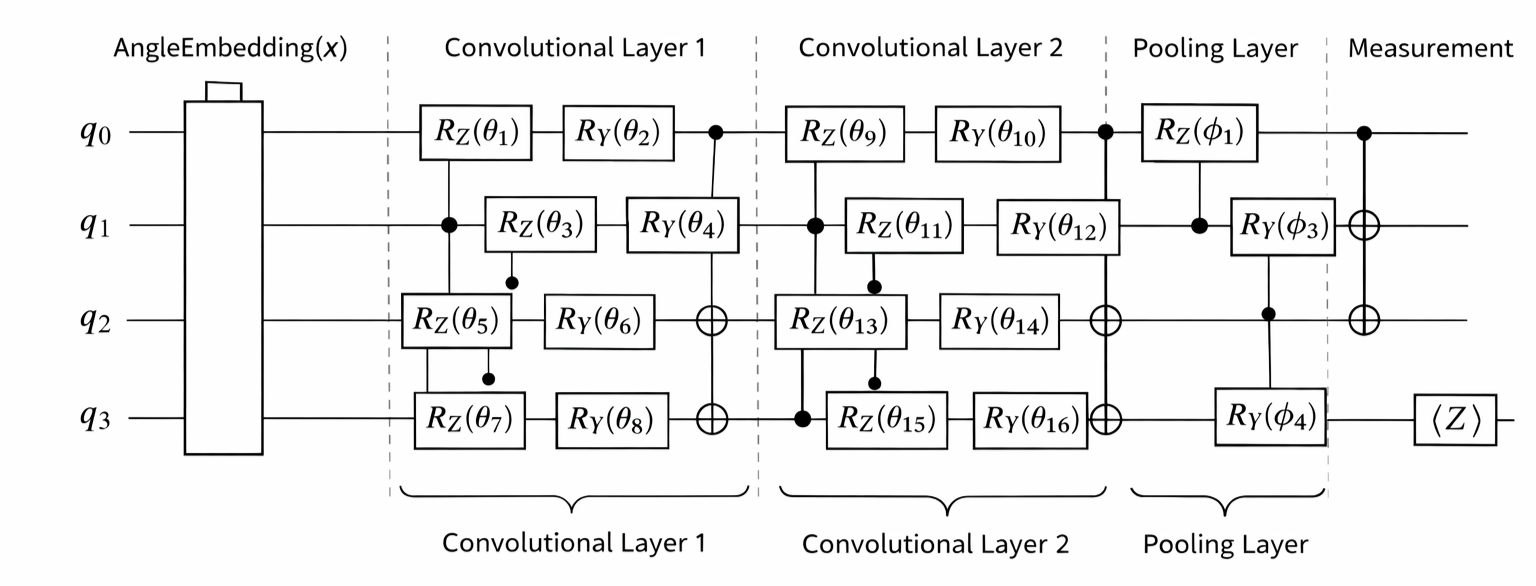
\includegraphics[width=0.8\textwidth]{imagens/Quantum_Circuit.png}
					
					%%%%%%%%%%%%%%%%      
				\end{block}
				
				
				\begin{block}{Quantum Advantages}
					
					\begin{itemize}
						
						\item \textbf{Reduced Dataset Requirements} - Quantum Neural Networks are known to produce effective predictive models with excellent generalization performance even when provided with only a small amount of training data. Leveraging High-dimensional Hilbert spaces and exponentially large state representations allow for this. 
						 
						
						\item \textbf{Resilience to Noise} - QCNNs can have improved performance in dealing with noisy ECG signal samples. Variational quantum circuits can exhibit robustness to certain types of noise due to the fact that they distribute information across amplitudes rather than store them deterministically.
					\end{itemize}
				\end{block}
				
				
				\begin{exampleblock}{Future Potential Research}
					While quantum convolutional neural networks have been proven to be somewhat effective in my past research when tasked with binary classification for normal vs Atrial Fibrillation (AF) ECG signals, when tasked with multi-classification my current model is not effective. Through further exploration of quantum circuit configurations and dimensionality reduction, a higher performing quantum model is achievable, however simulation and hardware restrictions make this challenging. 
				\end{exampleblock}
				
				\begin{block}{Acknowledgments}
					\begin{thebibliography}{9}
						
						\bibitem{statista}
						Statista. (n.d.). \textit{Deaths from leading causes of death in the United States}. 
						Available: https://www.statista.com/chart/30883/deaths-from-leading-causes-of-death-in-the-united-states/
						
						\bibitem{vu2023}
						T. Vu, T. Petty, K. Yakut, M. Usman, W. Xue, F. M. Haas, R. A. Hirsh, and X. Zhao, 
						``Real-time arrhythmia detection using convolutional neural networks,'' 
						\textit{Frontiers in Big Data}, vol. 6, 1270756, 2023. 
						doi: 10.3389/fdata.2023.1270756
						
						\bibitem{zheng2022}
						J. Zheng, H. Guo, and H. Chu, 
						``A large scale 12-lead electrocardiogram database for arrhythmia study (version 1.0.0),'' 
						\textit{PhysioNet}, 2022. 
						doi: 10.13026/wgex-er52
						
					\end{thebibliography}
				\end{block}
				
				%\begin{block}{References}
				%\nocite{*}
				%\bibliographystyle{plain}\bibliography{poster}
				%\end{block}
				
			\end{column}
			
			\separatorcolumn
		\end{columns}
	\end{frame}
	
\end{document}